\subsection{Funktionsbeschreibung}
Der Ballwerfer befindet sich in der Ausgangsposition in der Startfeldmitte. 
Nach einer drahtlosen Übermittlung des Startsignals beginnt das Smartphone auf 
dem Ballwerfer mit der Korberkennung. Zeitgleich werden die Schwungräder auf 
ihre Nenndrehzahl beschleunigt. Durch die Auswertung des fotografierten Bildes 
wird die Position des Korbes ermittelt und aus dieser einen Winkel für die 
Justierung der Abwurfeinheit des Ballwerfers berechnet.\\
\\
Nach der Übermittlung des Winkels an den Controller richtet der Stellantrieb 
die Abwurfeinheit in die gewünschte Wurfposition aus. Ein Förderband führt 
anschliessend die Bälle den Schwungrädern zu, wo diese auf ihre 
Abwurfgeschwindigkeit beschleunigt werden. Die Bälle verlassen nacheinander 
das Gerät und fliegen in einer Wurfparabel direkt in den Korb. Sobald sich 
alle Bälle im Korb befinden (zeitbedingt), wird das akustische Endsignal 
auf dem Smartphone ausgegeben.\\
\\
Die Grafik in Abbildung \ref{fig:FlowChart} stellt den 
schematischen Ablauf der oben erwähnten Funktionen dar. Einige Teilschritte 
des Ablaufes, wie zum Beispiel das Beschleunigen der Schwungräder, werden 
je nach zeitlicher Dauer oder möglicher auftretenden Störungen (in Form von 
Vibrationen) verschoben.
%
\begin{figure}[h!]
	\centering
	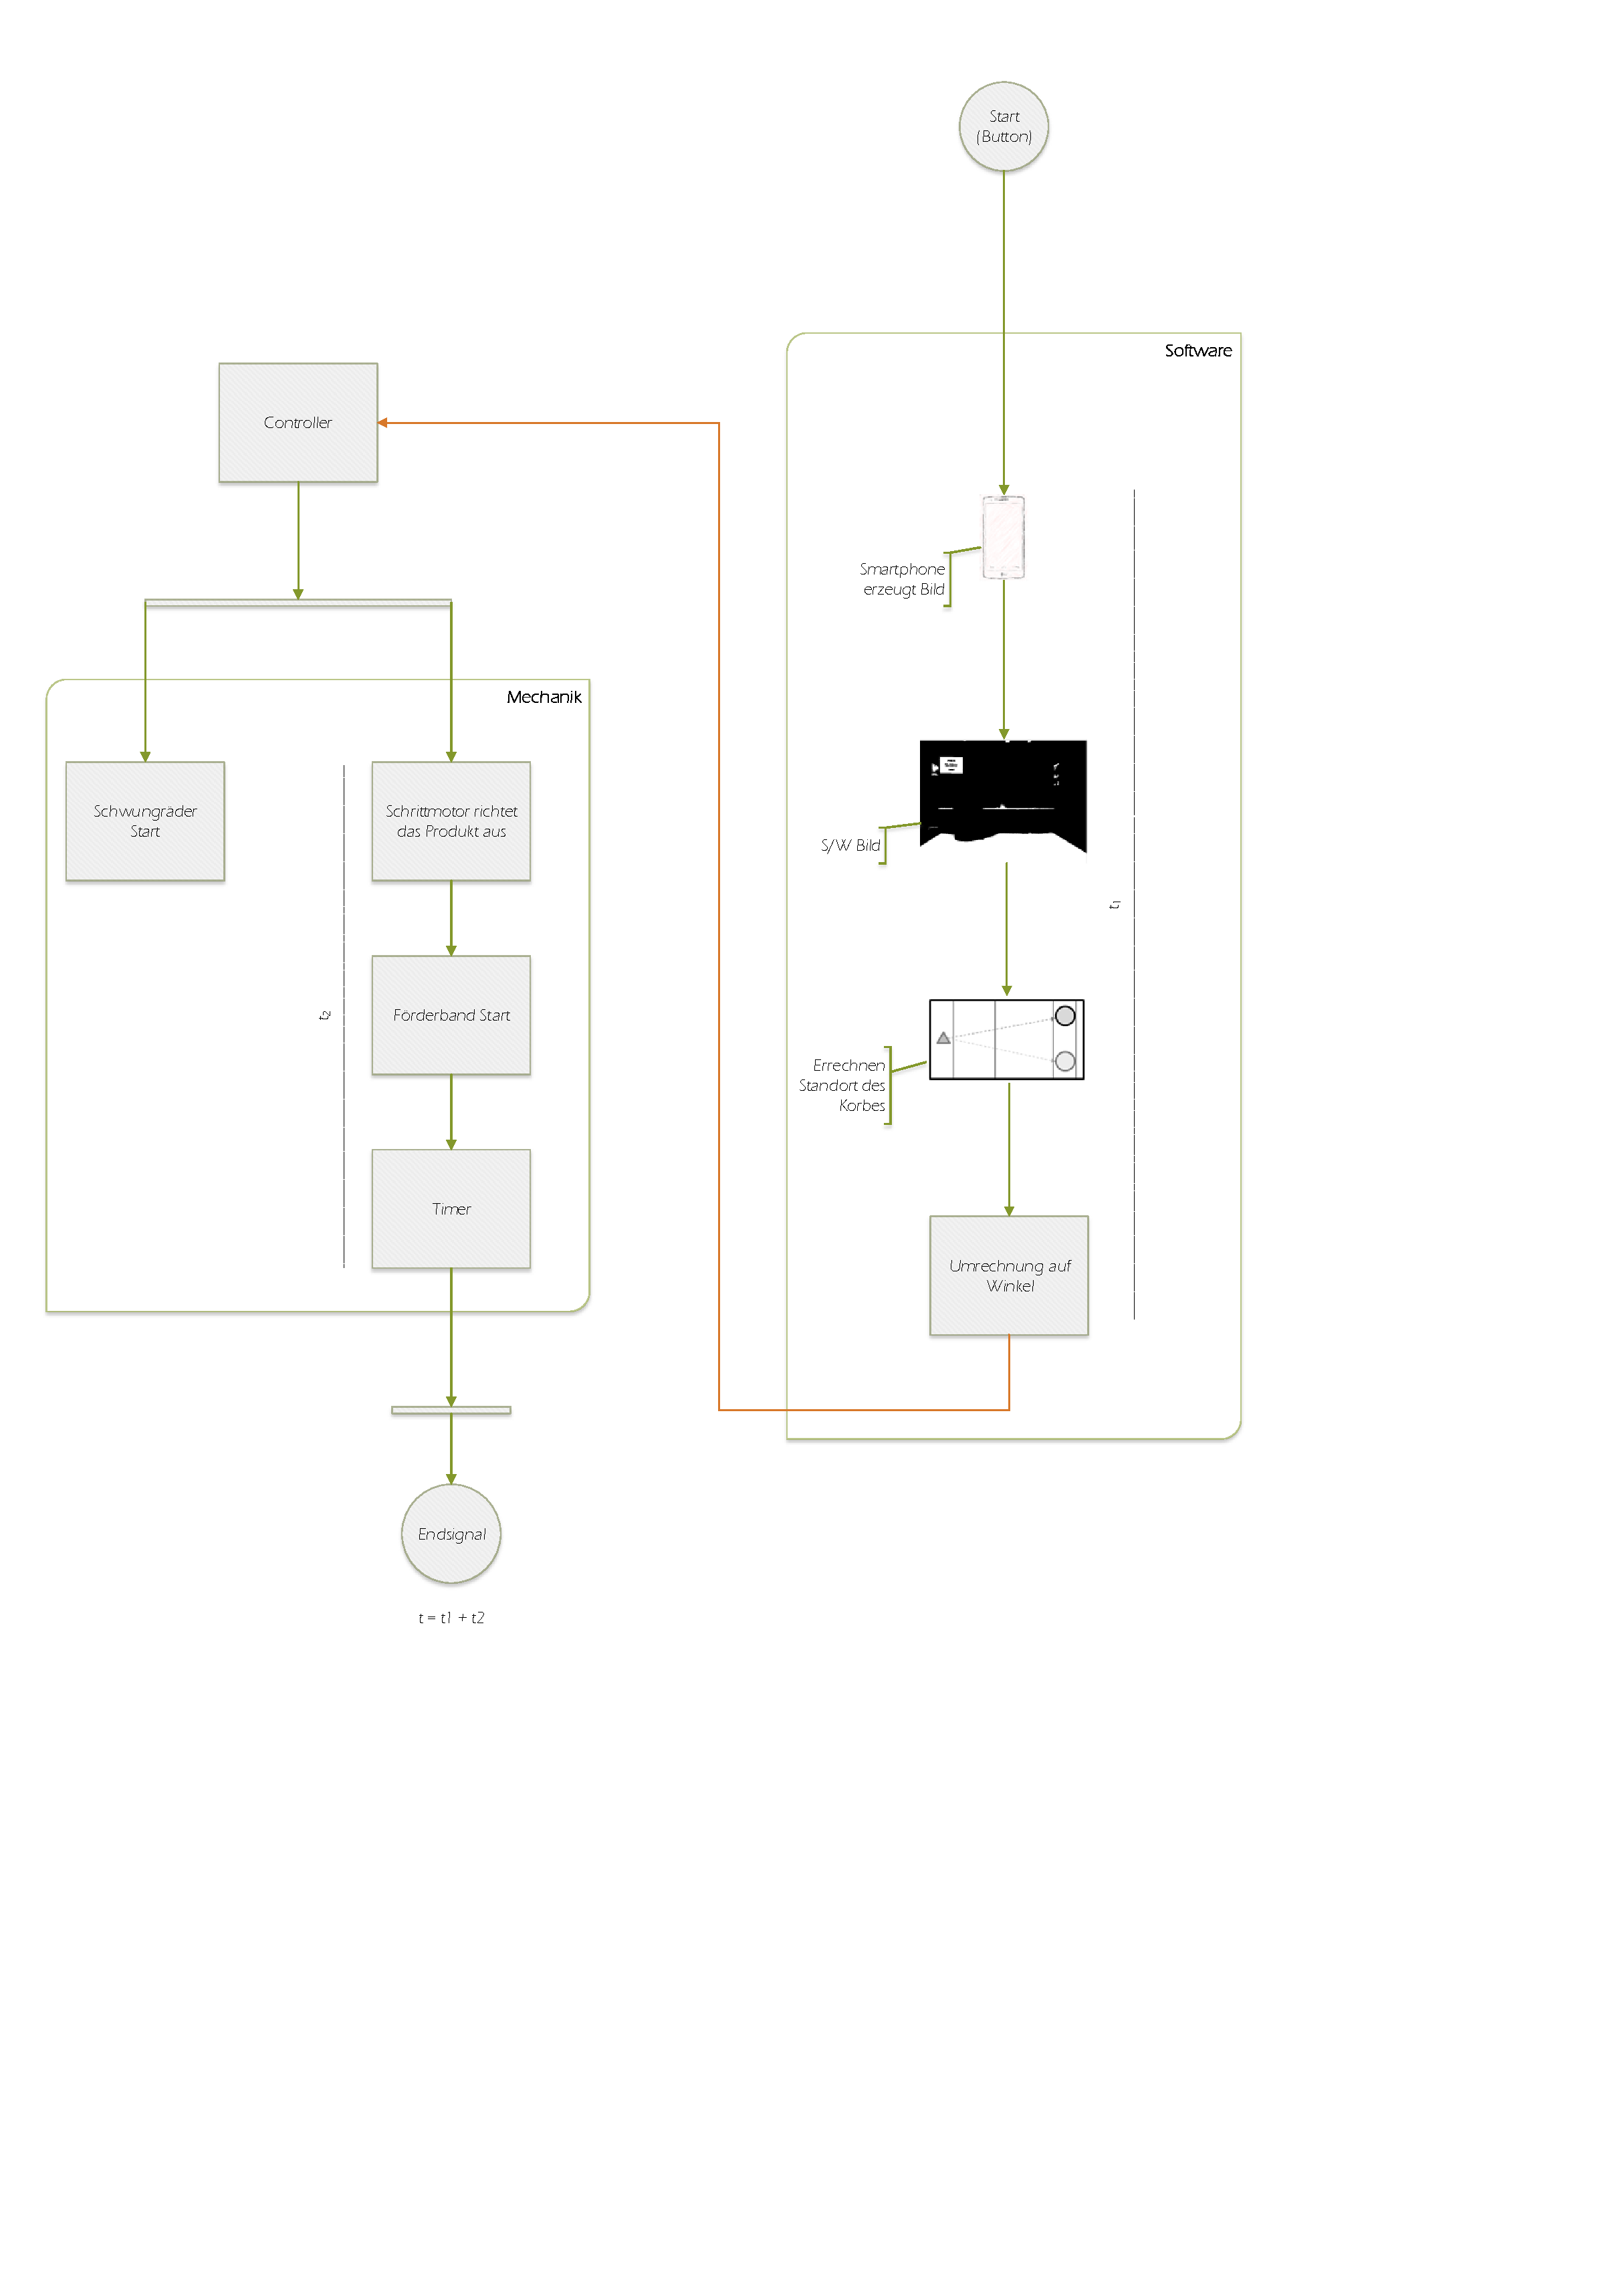
\includegraphics[width=1\textwidth,clip,trim=10mm 169mm 89mm 15mm]
	{Enddokumentation/Loesungskonzept/Bilder/FlowOnChart_v3.pdf}
	\caption{Ablaufdiagramm zur Funktionsbeschreibung}
	\label{fig:FlowChart}
\end{figure}
\clearpage